\chapter{Discusi\'on} 
\label{ch:discusion}

A lo largo de este trabajo presentamos como parcelar la corteza cerebral
en base a un criterio estructural; estudiamos una de las m\'etodos
existentes actuales y presentamos un m\'etodo pr\'opio. En los capitulos
1 y 2 introdujimos la parcelaci\'on estructural y sus fundamentos 
te\'oricos. En las secciones \ref{sec:clustering_moreno} y 
\ref{sec:analisis_moreno} analizamos el reciente aporte de 
Moreno-Dominguez \cite{Moreno-Dominguez2014} al estado del arte. El mismo
se basa en combinar un algoritmo de tractograf\'ia y otro de 
\textit{clustering} para parcelar la corteza cerebral. Luego, bas\`andonos
en su trabajo, propusimos en la secci\'on \label{ch:nuestro} un nuevo
algoritmo de \textit{clustering}. En este \'ultimo capitulo discutiremos
los resultados obtenidos durante este trabajo. Comenzando por la robustes
del algoritmo de tractograf\'ia utilizado; siguiendo con una comparaci\'on
entre nuestro m\'etodo y el de Moreno-Dominguez; continuando con la 
validez biol\'ogica de la parcelaci\'on obtenida y propondremos objetos de
futuro estudio. \\

\section{Convergencia del algoritmo de tractograf\'ia}

Creamos los tractogramas usando el algoritmo \ref{alg:itract} de la 
secci\'on \ref{sec:convergencia}. Los tractogramas creados de esta manera
son inherentemente estoc\'asticos. Implementamos el algoritmo 
\ref{alg:bootstrap} de la secci\'on \ref{sec:convergencia} para estudiar
si la creaci\'on de los tractogramas era estable. Esto es, si dado un 
n\'umero suficientemente grande de part\'iculas el resultado converge
a un \'unico tractograma. \\

El algoritmo utilizado en el trabajo demostr\'o ser estable. Las figuras 
\ref{fig:s1}, \ref{fig:s2} y \ref{fig:s3} de la secci\'on 
\ref{sec:resultado_estabilidad} muestran que la desviaci\'on est\'andar es
casi nula al usar $15000$ part\'iculas. A su vez, la figura \ref{fig:mv}
muestra lo r\'apido que converge la media de tres voxels distintos. 
Como eran los de mayor desv\'iacion est\'andar, podemos asegurar que casi
no existe diferencia en la media de los tractogramas creados con dos mil
part\'iculas. \\

Nuestro m\'etodo de parcelamiento se basa en el clustering de 
tractogramas. Por ello es importante contar con un algoritmo de 
tractograf\'ia robusto. No encontramos estudios previos donde se analizara
este aspecto del algoritmo de tractograf\'ia usado. \\


\section{Comparaci\'on entra ambos m\'etodos de $clustering$}

En la secci\'on \ref{sec:clustering_moreno} presentamos el m\'etodo para
parcelar la corteza de Moreno-Dominguez. Luego, en la secci\'on
\label{ch:nuestro} presentamos nuestro m\'etodo. El resultado de parcelar
el \'area de Broca con estos se pueden ver en las secciones 
\ref{sec:moreno_broca} y \ref{sec:nuestro_broca}. En la secci\'on 
\label{sec:acercamiento} presentamos los resultados lado a lado en detalle
para compararlos. Los resultados son visualmente parecidos en todos los
casos. \\

Luego utilizamos ambos algoritmo para parcelar el hemisferio izquierdo del
mismo sujeto. Los resultados se encuentran en las secciones 
\label{sec:corteza_moreno} y \label{sec:corteza_nuestro}. En este caso 
resulta dif\'icil comparar visualmente las parcelaciones. M\'as a\'un, es
complicado encontrar cortes en los dendrogramas que generen
representaciones parecidas. Dado que los arboles fueron generados
de manera distinta, sus cortes no tienen por que corresponderse. Sin
embargo, la secci\'on \ref{sec:acercamiento_corteza} muestra algunas
similitudes en: la corteza motora y la somest\'esica; el l\'obulo frontal;
el l\'obulo occipital y el \'area de Broca. \\

Respecto a la eficiencia computacional, en la secci\'on 
\ref{sec:nuestro_clustering} comparamos ambos m\'etodos. 
Mostramos que nuestro m\'etodo permite mejorar la complejidad temporal y
espacial en al menos un orden de magnitud. Nuestro algoritmo de clustering
posee complejidad espacial $O(s^2)$ contra $O(s^2 + sm)$ del m\'etodo
Moreno-Dominguez. La complejidad temporal de nuestro algoritmo es $O(s^2m)$
contra $O(s^2)$ del m\'etodo Moreno-Dominguez. Recordemos de la secci\'on
\ref{sec:ralas} que dentro del contexto de este trabajo $m >> s$. En
general el n\'umero de semillas usadas es muy menor a la cantidad de
voxels de los tractogramas. En nuestro caso particular $s \cong 22000$ y
$m \cong 3500000$. $m$ es $159$ veces mas grande que $s$. \\


\section{Correlato con otras parcelaciones de la literatura}

Nuestro m\'etodo divide la corteza cerebral bas\'andonse en el 
agrupamiento de tractogramas. El criterio usado es puramente estructural.
Solo usamos informaci\'on sobre la estructura f\'sica de la materia
blanca. En la literatura actual existen parcelaciones basadas en otros
criterios. Desikan et al. \cite{Desikan2006} dividen la corteza usando
como referencia las circunvoluciones del cerebro. Peinfield 
\cite{Penfield1954} parcela la corteza en base a las respuestas a 
est\'imulos el\'ectricos sobre la misma. La parcelaci\'on de Desikan es
anat\'omica, mientras que la de Peinfield es funcional. Una pregunta
interesante es si nuestra parcelaci\'on posee correlaci\'on con otras
anat\'omicas o funcionales. La relaci\'on entre el aspecto anat\'omico o
funcional del cerebro y su aspecto estructural es un problema abierto en
neurociencia.  En el trabajo de Moreno-Dominguez solo hacen una breve
comparaci\'on entre sus resultados y un mapa citoarquitect\'onico. A 
continuaci\'on contrastaremos nuestros resultados con un atlas anat\'omico
y un estudio funcional realizado sobre el sujeto.  \\


\subsection{Correlaci\'on anat\'omica}
\label{sec:corr_anatomica}

En la secci\'on \label{sec:corteza_nuestro} parcelamos el hemisferio 
izquiero de un sujeto con nuestro m\'etodo. Vamos a comparar nuestro
resultado con el atlas anat\'omico basado en Desikan et al. 
\cite{Desikan2006}. La figura \ref{fig:an2pa} muestra el resultado de proyectar algunas regiones anat\'omicas sobre las obtenidas con nuestro
m\'etodo. La figura \ref{fig:an2pa2} muestra solo las regiones que estaban
contenidas en su mayor\'ia dentro de estas proyecciones. Luego calculamos
que porcentaje de las parcelaciones quedaba dentro de las proyecciones;
que porcentaje quedaba fuera y cuantas quedaban dentro de una sola 
proyecci\'on. El $90\%$ del \'area de las 9 proyecciones est\'a pintada y
solo un $5\%$ del \'area de nuestras parcelas queda fuera de las
proyecciones. Las parcelas de nuestro m\'etodo que se encuentran en una
sola proyecci\'on representan el $88\%$ del \'area pintada. Las parcelas
que est\'an en dos regiones representan el $12\%$ restante. Esto indica
que casi todas nuestras parcelas se encuentran contenidas dentro de a lo
sumo una proyecci\'on. Nuestra parcelaci\'on cre\'o \'areas bien
delimitadas dentro de al menos 9 regiones anat\'omicas. \\

Repetimos este procedimiento de proyectar el atlas anat\'omico sobre la
parcelaci\'on obtenida en la figura \ref{fig:moreno_corteza2}. Dicha
parcelaci\'on fue obtenida mediante el m\'etodo de Moreno-Dominguez.
En este caso el $75\%$ del \'area de las 9 proyecciones est\'a pintada y 
un $15\%$ del \'area de las parcelas quedan fuera de las proyecciones. 
Sin embargo esto no quiere decir que el m\'etodo de Moreno-Dominguez 
posea menor correlaci\'on con el atlas anat\'omico. La parcelaci\'on 
resultante en ambos m\'etodos depende de la altura a la cual se decida 
cortar el dendrograma. Cortando el mismo dendrograma a mayor profundidad
se pueden conseguir resultados similares a los de nuestro m\'etodo.\\

\begin{figure}[h!]
    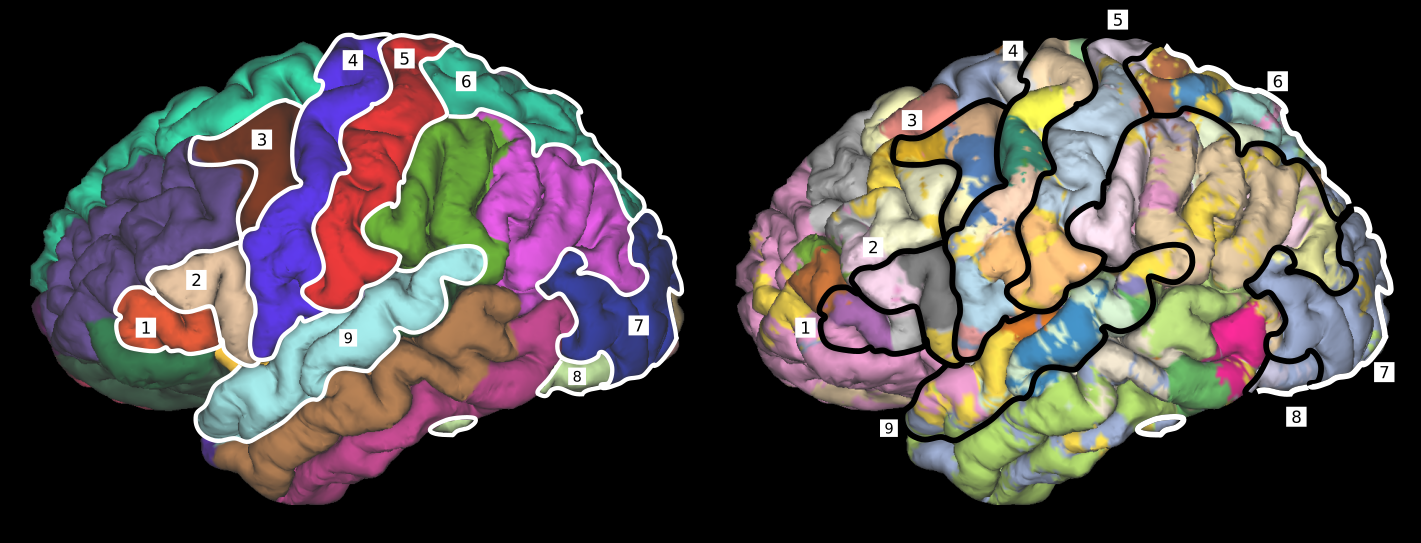
\includegraphics[width=\textwidth]{img/anatomica2parcelation.png}
    \caption{Proyecci\'on del atlas anat\'omico (izquierda) a la 
             parcelaci\'on obtenida (derecha). Regiones: 
             1. \textit{pars triangularis}; 2. \textit{pars opercularis};
             3. \textit{caudal middle frontal}; 
             4. \textit{precentral (\'area motora)}; 
             5. \textit{post central}; 6. \textit{superior parietal}; 
             7. \textit{lateral occipital}; 8. \textit{fusiform};
             9. \textit{superior temporal}.  }
    \label{fig:an2pa}
\end{figure}

\begin{figure}[h!]
    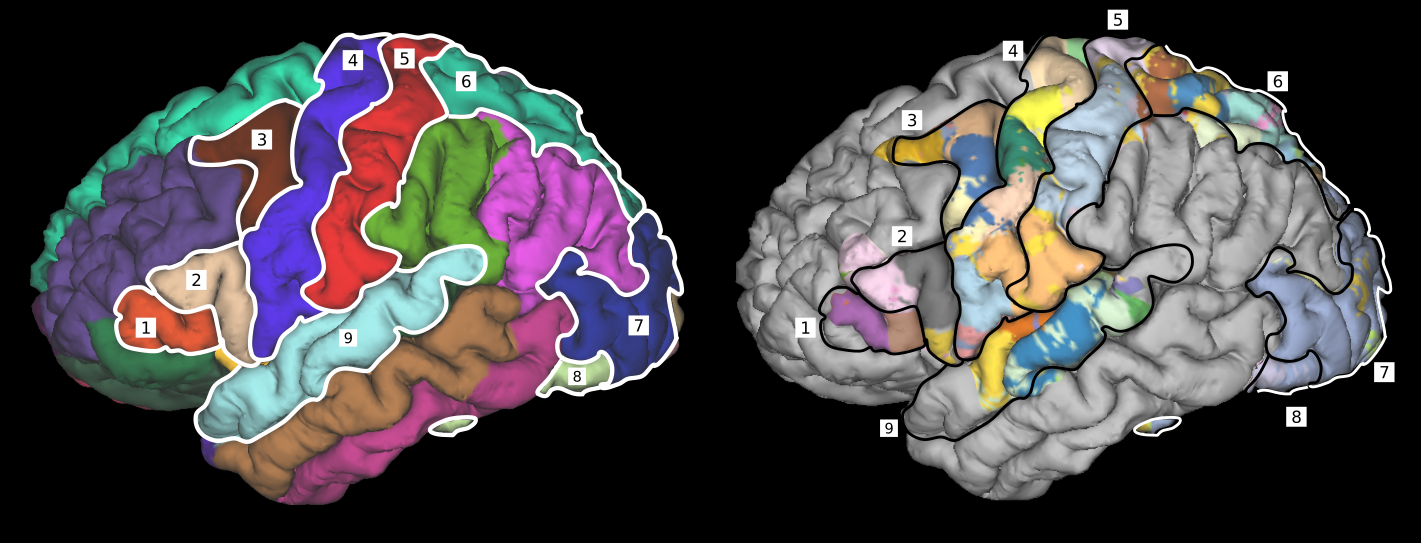
\includegraphics[width=\textwidth]{img/anatomica2parcelation2.png}
    \caption{Proyecci\'on del atlas anat\'omico (izquierda) a la 
             parcelaci\'on obtenida (derecha). Solo las parcelas contenidas
             en mayor proporci\'on fueron pintadas. Regiones: 
             1. \textit{pars triangularis}; 2. \textit{pars opercularis};
             3. \textit{caudal middle frontal}; 
             4. \textit{precentral (\'area motora)}; 
             5. \textit{post central}; 6. \textit{superior parietal}; 
             7. \textit{lateral occipital}; 8. \textit{fusiform};
             9. \textit{superior temporal}.  }
    \label{fig:an2pa2}
\end{figure}

\subsection{Correlaci\'on funcional}
\label{sec:corr_funcional}

El sujeto de \textit{Human Connectome Project} utilizado cuenta con un 
estudio funcional hecho por Bach et al. \cite{Barch2013}. En el mismo
utilizan Resonancia Magn\'etica Funcional (fMRI) para estudiar la
respuesta sobre la corteza a est\'imulos particulares. La Resonancia 
Magn\'etica Funcional es un tipo especial de resonancia magn\'etica que
mide el nivel de oxigeno en sangre \cite{Ogawa1990}. Nosotros nos
enfocamos en las respuestas a los siguientes est\'imulos: mover la mano;
mover el pie; mover la lengua; reconocer formas y caras vistas con
anterioridad; clasificar un cuento breve dentro de dos categor\'ias y
resolver problemas aritm\'eticos simples. Por cada uno de estos
est\'imulos se cuenta con un mapa de \textit{z-scores} sobre la corteza.
Estos \textit{z-scores} representan la correlaci\'on entre la activaci\'on
de cada punto de la corteza con el est\'imulo. \\

\begin{figure}[h!]
    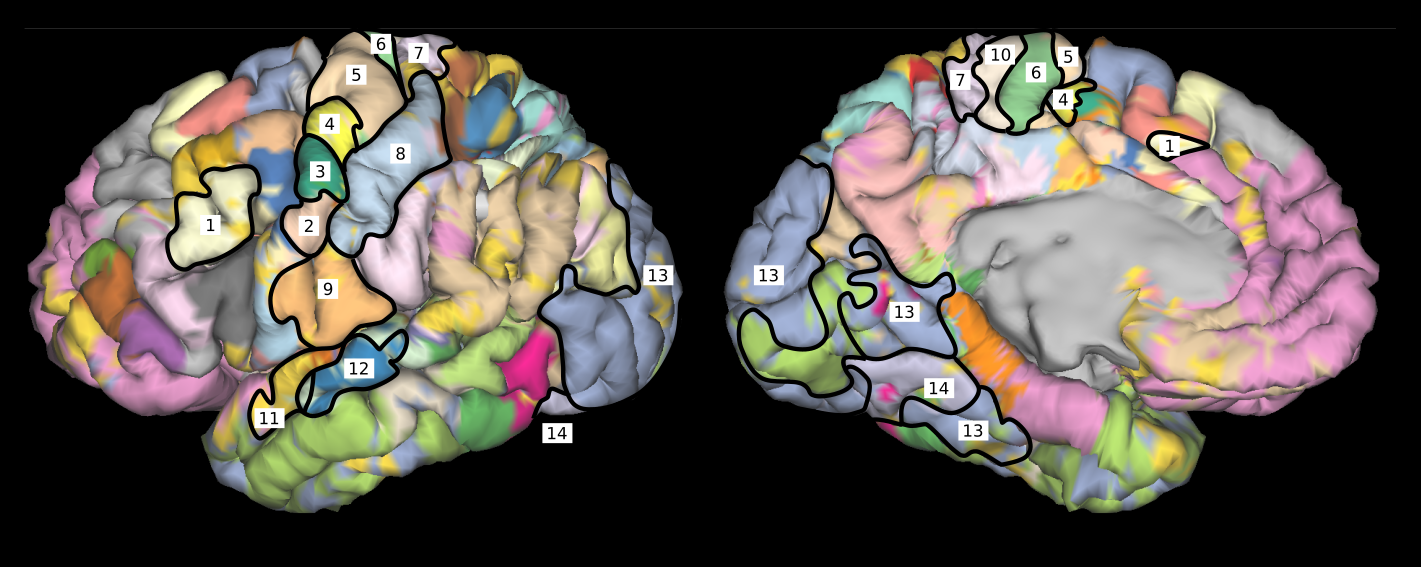
\includegraphics[width=\textwidth]{img/32k_labels.png}
    \caption{Parcelas en baja resoluci\'on}
    \label{fig:32k}
\end{figure}


\begin{figure}[h!]
    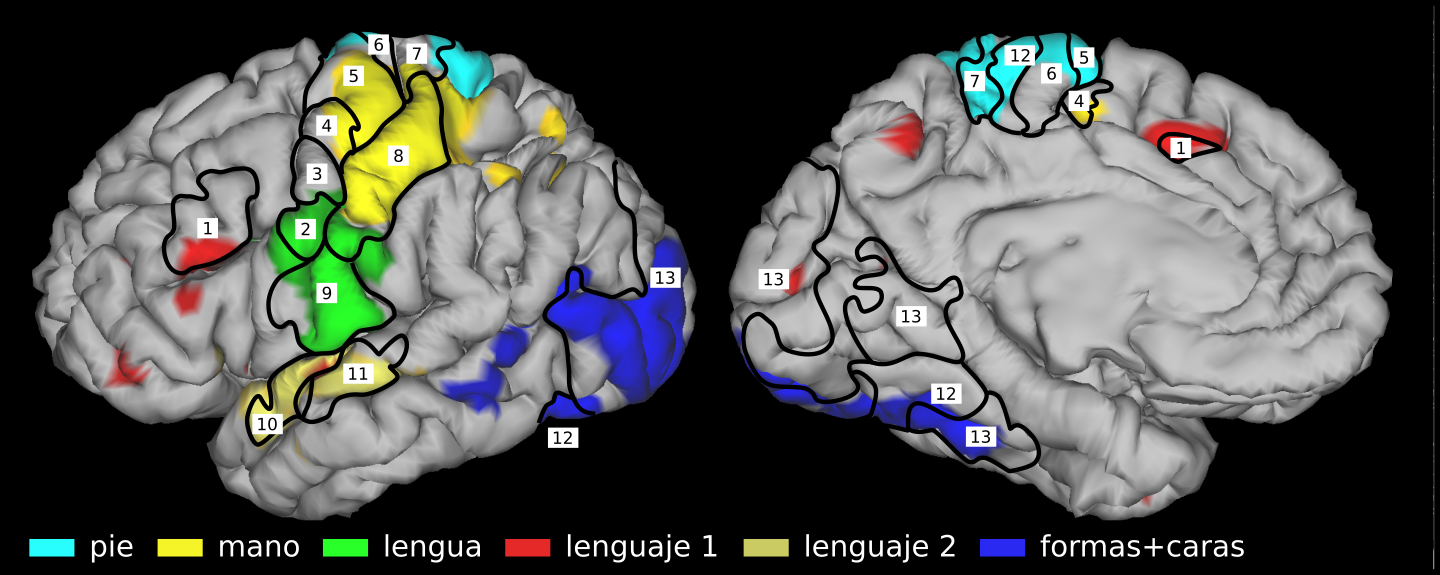
\includegraphics[width=\textwidth]{img/32k_z5.png}
    \caption{Projecci\'on de las parcelas (izquierda) sobre los \textit{z-scores}
    mayores a $5$ de las activaciones funcionales (derecha)}
    \label{fig:32k_z5}
\end{figure}

\begin{figure}[h!]
    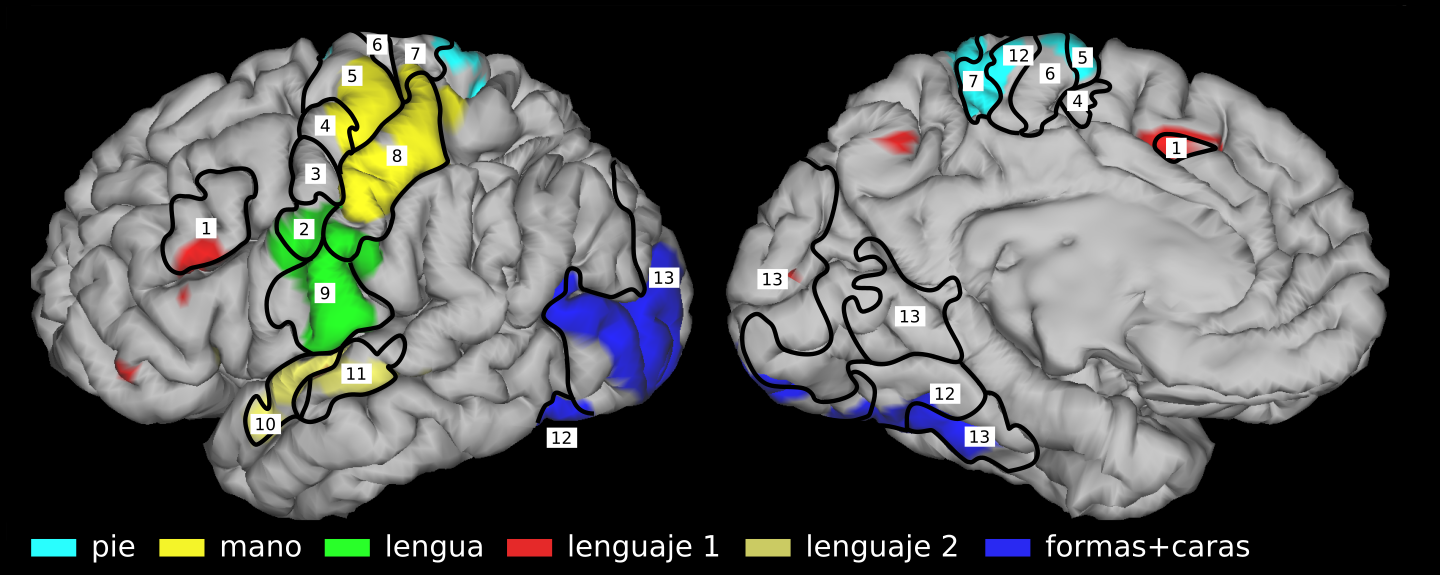
\includegraphics[width=\textwidth]{img/32k_z7.png}
    \caption{Projecci\'on de las parcelas (izquierda) sobre los \textit{z-scores}
    mayores a $7$ de las activaciones funcionales (derecha)}
    \label{fig:32k_z7}
\end{figure}


Queremos comparar los mapas de \textit{z-scores} con una de las 
parcelaciones obtenidas mediante nuestro m\'etodo. Para ello primero
interpolamos la parcelaci\'on utilizada en la secci\'on anterior a la
superficie en que se encuentran los mapas. El resultado de dicha 
interpolaci\'on puede verse en la figura \ref{fig:32k}. Algunas regiones
de inter\'es fueron etiquetadas. La figura \ref{fig:32k_z5} muestra la
proyecci\'on de estas regiones sobre los \textit{z-scores} $ \geq 5$ de
los distintos mapas. La figura \ref{fig:32k_z7} muestra la proyecci\'on
sobre los \textit{z-scores} $ \geq 7$. Luego definimos la siguiente 
m\'etrica entre superficies: \\

$$ superposicion(A,B) = \frac{ 2 * area(A \cap B) }{area(A) + area(B)} $$ 
 
Dadas dos superficies $A$ y $B$ se cumple: 
$0 \leq superposicion(A,B) \leq 1$. El $0$ representa que son superficies
disjuntas y el $1$ que est\'an totalmente superpuestas. La tabla 
\ref{tb:zscore5} muestra la superposici\'on entre las superficies de 
nuestra parcelaci\'on y los \textit{z-scores} $ \geq 5$.  La tabla 
\ref{tb:zscore7} muestra la superposici\'on entre las superficies de 
nuestra parcelaci\'on y los \textit{z-scores} $ \geq 7$. En cada columna
se resalt\'o el valor mas grande. Esto es, el valor de la parcela que
mayor superficie compart\'ia con cada mapa de activaci\'on.  \\
 
\begin{table}[]
\centering
\begin{tabular}{|l|l|l|l|l|l|l|}
\hline
   & pie   & mano  & lengua & matemática & cuento & formas \\ \hline
1  & 0     & 0     & 0      & 0.276      & 0      & 0      \\ \hline
2  & 0     & 0     & 0.311  & 0          & 0      & 0      \\ \hline
3  & 0     & 0     & 0      & 0          & 0      & 0      \\ \hline
4  & 0     & 0.172 & 0      & 0          & 0      & 0      \\ \hline
5  & 0.177 & 0.321 & 0      & 0          & 0      & 0      \\ \hline
6  & 0.201 & 0     & 0      & 0          & 0      & 0      \\ \hline
7  & 0.231 & 0.044 & 0      & 0          & 0      & 0      \\ \hline
8  & 0     & {\bf 0.590} & 0.139  & 0          & 0      & 0      \\ \hline
9  & 0     & 0     & {\bf 0.610}   & 0          & 0      & 0      \\ \hline
10 & {\bf 0.330}  & 0     & 0      & 0          & 0      & 0      \\ \hline
11 & 0     & 0     & 0      & 0          & {\bf 0.606}  & 0      \\ \hline
12 & 0     & 0     & 0      & 0          & 0.454  & 0      \\ \hline
13 & 0     & 0     & 0      & 0          & 0      & {\bf 0.491}  \\ \hline
14 & 0     & 0     & 0      & 0          & 0      & 0.154  \\ \hline
\end{tabular}
\caption{Relaci\'on entre las \'areas de cada parcela y los mapas de
         activaci\'on con $zscore > 5$. Los valores m\'aximos de cada 
         columna fueron resaltados.}
\label{tb:zscore5}         
\end{table}


\begin{table}[]
\centering

\begin{tabular}{|l|l|l|l|l|l|l|}
\hline
   & pie   & mano  & lengua & matemática & cuento & formas \\ \hline
1  & 0     & 0     & 0      & {\bf 0.419} & 0     & 0      \\ \hline
2  & 0     & 0     & 0.323  & 0          & 0      & 0      \\ \hline
3  & 0     & 0     & 0      & 0          & 0      & 0      \\ \hline
4  & 0     & 0.115 & 0      & 0          & 0      & 0      \\ \hline
5  & 0.141 & 0.341 & 0      & 0          & 0      & 0      \\ \hline
6  & 0.095 & 0     & 0      & 0          & 0      & 0      \\ \hline
7  & {\bf 0.377} & 0.040 & 0      & 0          & 0      & 0      \\ \hline
8  & 0     & {\bf 0.669} & 0.147  & 0          & 0      & 0      \\ \hline
9  & 0     & 0     & {\bf 0.629}  & 0          & 0      & 0      \\ \hline
10 & 0.240 & 0     & 0      & 0          & 0      & 0      \\ \hline
11 & 0     & 0     & 0      & 0          & {\bf 0.715}  & 0      \\ \hline
12 & 0     & 0     & 0      & 0          & 0.458  & 0      \\ \hline
13 & 0     & 0     & 0      & 0          & 0      & {\bf 0.428}  \\ \hline
14 & 0     & 0     & 0      & 0          & 0      & 0.154 \\ \hline
\end{tabular}
\caption{Relaci\'on entre las \'areas de cada parcela y los mapas de
         activaci\'on con $zscore > 7$. Los valores m\'aximos de cada 
         columna fueron resaltados.}
\label{tb:zscore7}         
\end{table}

En los \'items \ref{sec:corr_anatomica} y \ref{sec:corr_funcional} 
comparamos la parcelaci\'on obtenida por nuestro m\'etodo contra
un atlas anat\'omico y un estudio funcional del sujeto. Veamos una por 
una las secciones etiquetadas en la figura \ref{fig:32k}. Los resultados
muestran que la regi\'on $1$ es funcionalmente consistente con la 
resoluci\'on de problemas matem\'aticos. Las regiones $2-10$ son consistentes anat\'omicamente con la corteza motora. A su vez, tambi\'en son consistentes con el hom\'unculo cortical .El hom\'unculo cortical,
definido por Penfield \cite{Penfield1954}, es una divisi\'on funcional de
la corteza motora y de la corteza somastest\'esica. Mapea distintas 
regiones del cuerpo con regiones de la corteza como puede verse en la
figura \ref{fig:homunculo}. Las regiones $11$ y $12$ son consistentes 
anat\'omica y funcionalmente con el l\'obulo temporal superior.
Finalmente, las regiones $13$ y $14$ son consistentes anat\'omica y
funcionalmente con el l\'obulo occipital. Estos resultados son prometedores
y motivan a seguir estudiando el m\'etodo propuesto.

\begin{figure}[h!]
    \centering
    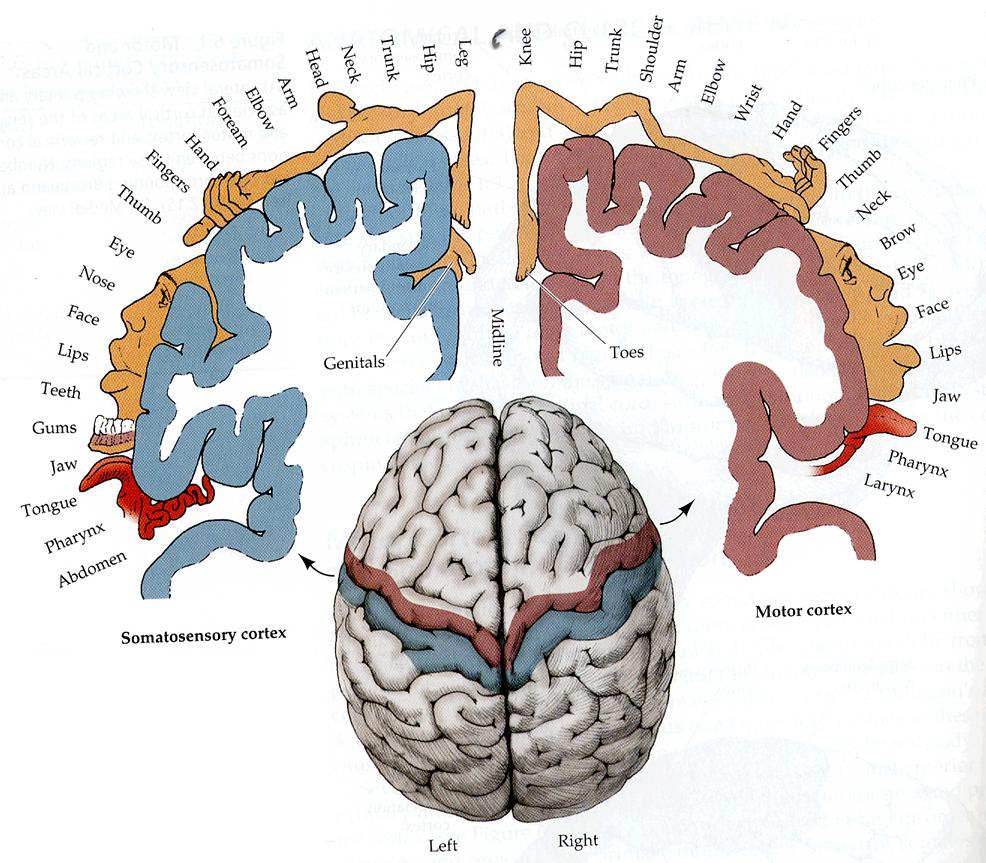
\includegraphics[width=0.8\textwidth]{img/homunculus.jpg}
    \caption{Hom\'unculo Cortical}
    \label{fig:homunculo}
\end{figure}

\section{Trabajo Futuro}
En este trabajo presentamos un nuevo m\'etodo para parcelar la corteza
cerebral mediante el agrupamiento de tractogramas. El m\'etodo mostr\'o
resultados con una fuerte correlaci\'on anat\'omica y funcional sobre el
sujeto estudiado. Por eso es importante seguir estudiando algunos aspectos
del proceso de parcelamiento. Primero, en este trabajo generamos 
tractogramas utilizando el algoritmo \ref{alg:itract} de la secci\'on 
\label{sec:convergencia}. Ser\'ia interesante estudiar los resultados
que se obtienen al usar otros algoritmos de tractograf\'ia. Segundo, 
en las secciones \label{sec:clustering_moreno} y \label{sec:nuestro_clustering} se puede ver que ambos m\'etodos de $clustering$
cuentan con un par\'ametro $k$. Este par\'ametro indica la cantidad de iteraciones a realizar uniendo solo $clusters$ vecinos y de tema\~no
similar. En el trabajo de Moreno-Dominguez \cite{Moreno-Dominguez2014} 
muestran una forma de calcular dicho par\'ametro para su m\'etodo. Hay
que estudiar una forma de calcularlo para el nuestro. Tercero, habr\'ia
que aplicar el m\'etodo sobre una poblaci\'on de sujetos y ver su
estabilidad. Esto es, estudiar si los resultados son igual de buenos que
con el sujeto aqu\'i elegido. Finalmente, en la secci\'on 
\label{sec:logit} mostramos que es posible aplicar operaciones
lineales en el espacio $LogOdds$. Esto puede utilizarse en particular para
calcular el tractograma medio de una poblaci\'on de sujetos. Hay que 
analizar si esto permite crear un atlas de la corteza basado solo en
informaci\'on estructural.

